\documentclass[a4wide,10pt]{article}

\usepackage[english]{babel}
\usepackage{graphicx}
\usepackage{tabu}
\usepackage{rotating}
\usepackage{multirow}
\usepackage[compatibility=false,labelfont=bf,center,justification=centering]{caption}
\usepackage{verbatim}
\usepackage[font=scriptsize]{subcaption}
\usepackage{changepage}
\usepackage{textpos}
\usepackage{booktabs}
\usepackage{dcolumn}
\usepackage{tikz}
\usetikzlibrary{calc}
\usepackage[compat=1.0.0]{tikz-feynman}
\usepackage{xspace}
\usepackage[margin=0.3in]{geometry}
\usepackage{epstopdf}

\begin{document}
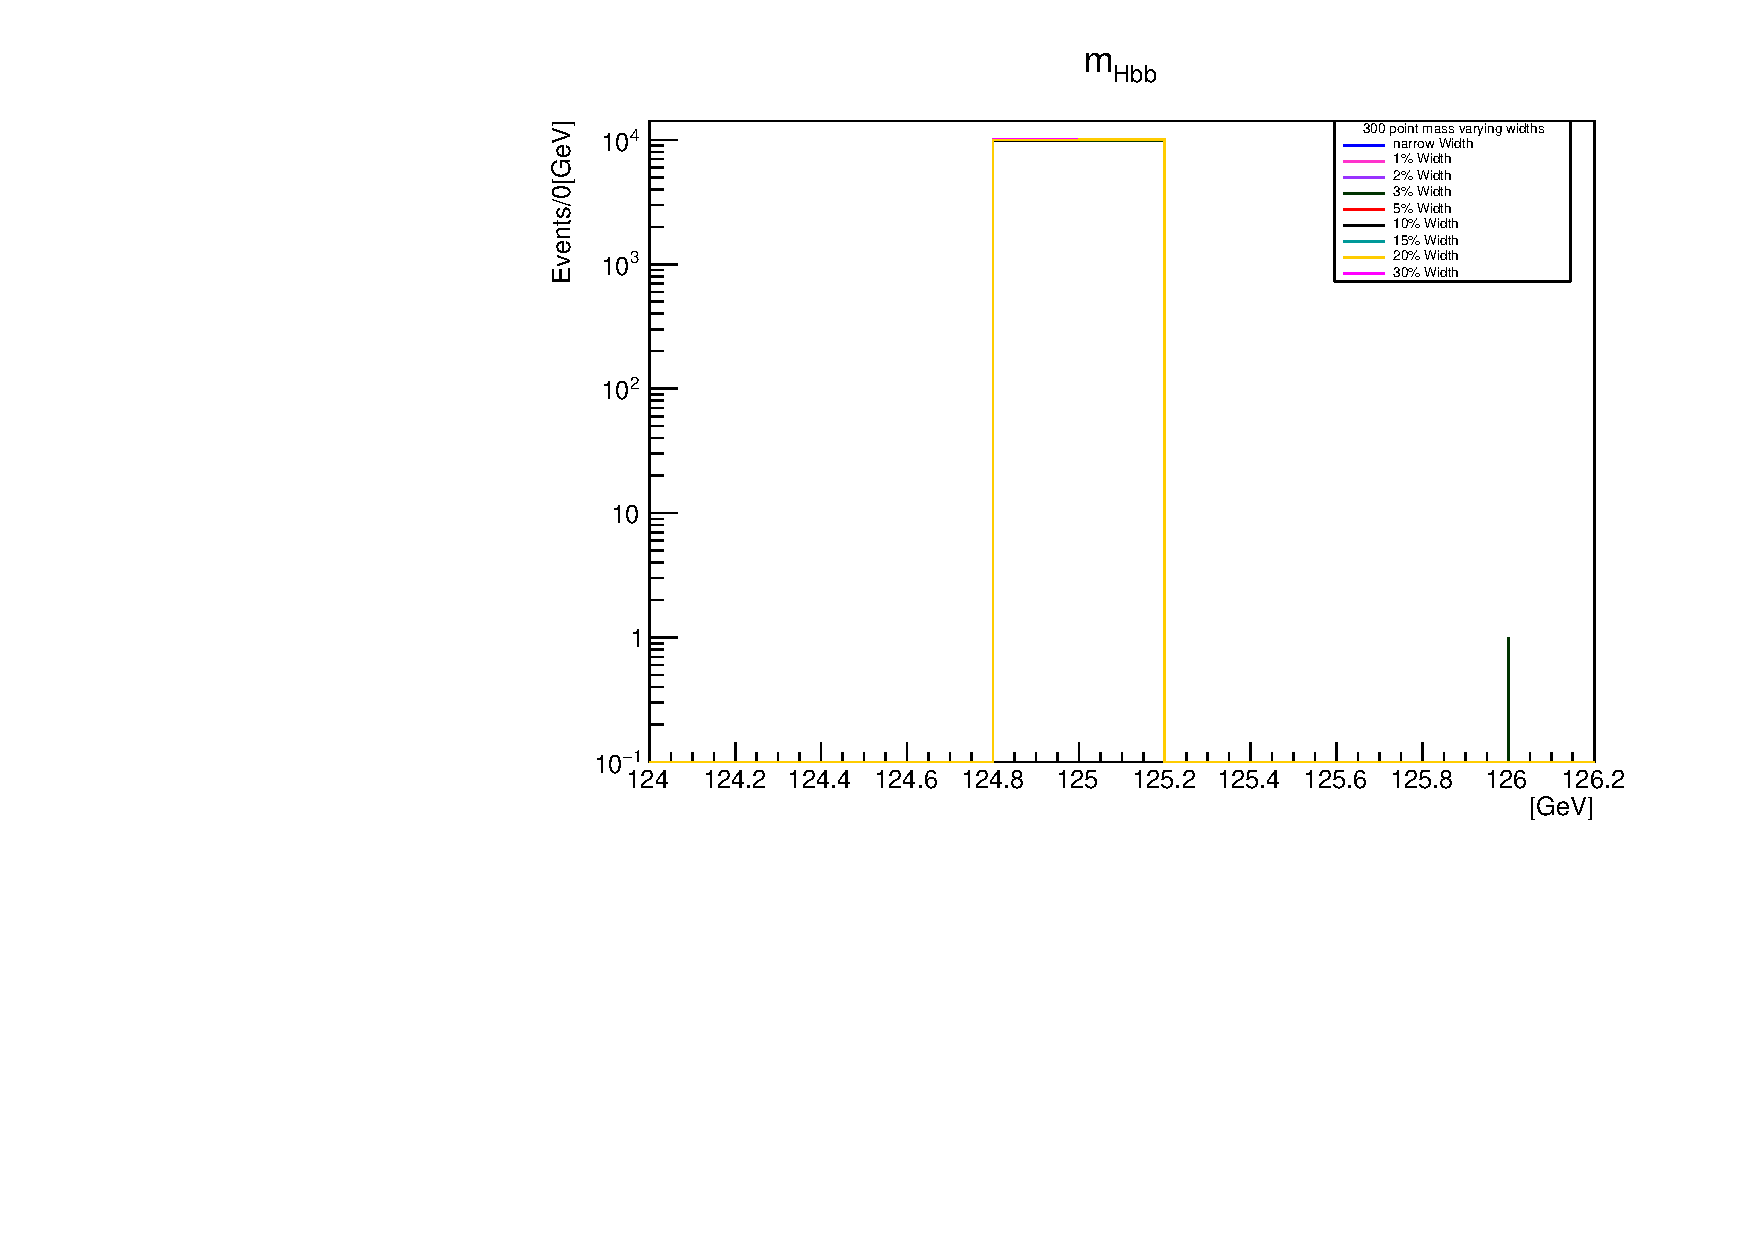
\includegraphics[scale=0.50,page=1]{../Pdfs/Hbb_Mass_VaryingWidths.pdf}
\includegraphics[scale=0.50,page=2]{../Pdfs/Hbb_Mass_VaryingWidths.pdf}
\includegraphics[scale=0.50,page=3]{../Pdfs/Hbb_Mass_VaryingWidths.pdf}
\includegraphics[scale=0.50,page=4]{../Pdfs/Hbb_Mass_VaryingWidths.pdf}
\includegraphics[scale=0.50,page=5]{../Pdfs/Hbb_Mass_VaryingWidths.pdf}
\includegraphics[scale=0.50,page=6]{../Pdfs/Hbb_Mass_VaryingWidths.pdf}
\includegraphics[scale=0.50,page=7]{../Pdfs/Hbb_Mass_VaryingWidths.pdf}
\includegraphics[scale=0.50,page=8]{../Pdfs/Hbb_Mass_VaryingWidths.pdf}
\includegraphics[scale=0.50,page=9]{../Pdfs/Hbb_Mass_VaryingWidths.pdf}
\includegraphics[scale=0.50,page=10]{../Pdfs/Hbb_Mass_VaryingWidths.pdf}
\includegraphics[scale=0.50,page=11]{../Pdfs/Hbb_Mass_VaryingWidths.pdf}
\includegraphics[scale=0.50,page=12]{../Pdfs/Hbb_Mass_VaryingWidths.pdf}
\includegraphics[scale=0.50,page=13]{../Pdfs/Hbb_Mass_VaryingWidths.pdf}
\includegraphics[scale=0.50,page=14]{../Pdfs/Hbb_Mass_VaryingWidths.pdf}

\end{document}Hbb_Mass_VaryingWidths.pdf